\section{Evaluation}\label{sec:evaluation}


\subsection{Experimental Setup}

We implement SwitchBox on a Hardkernel Odroid XU3 ARM big.LITTLE system with
Samsung Exynos 5422 A15/A7 heterogeneous multi-processing quad core CPUs at
maximum clock speed, 2 gigabyte LPDDR3 RAM at 933 MHz, and an eMMC5.0 HS400
backing store running Ubuntu Trusty 14.04.6 LTS, kernel version 3.10.106.

The maximum theoretical memory bandwidth for this model is 14.9GB/s\@.
Our observed maximum memory bandwidth is 4.5GB/s. \TODO{I think you
  need to sy that you are using a ram drive, right? Probably before
  you mention the memory bandwidth.  Also, this setup section needs to
  describe all of the different workloads you use and why; i.e., what
  they are representative of.}

\subsection{Experimental Methodology}
In this section we answer the following questions:
\begin{enumerate}
 \item Does incorporation of cipher-switching change the threat analysis? 
 \item Can SwitchBox reach security/energy tradeoffs that are not reachable with prior work?
 \item What switching strategy works best in which scenario? For which workload?
 \item What is the performance overhead of each cipher switching strategy?
 \item What is the storage overhead of each cipher switching strategy?
\end{enumerate}

\TODO{ Each of these quetions should become a subsection (although you
  might just have a single overhead subsection, rather than two. Also,
  I really want a security analysis section in the evaluation, and I
  added a first question to cover that.  I think you can basically reuse the table from the strongbox paper, but have a different column for forward, selective, and mirrored. }

\TODO{As I read through what is in here now, I also realize there needs to be some discussion of the different sizes and how they relate.  I would prefer one exhaustive set of charts and then something that says these trends are similar across workloads, so from now on we just focus on 40MB or something. Or if there is a really significant difference for different workloads, then we will have to show different sizes and you will need to justify that choice.}

\TODO{(see LaTeX source for some hidden charts here)}

\TODO{This section still needs a lot of work.  Right now, even the outline of the section is unclear.  I expect a subsection for each of the questions above.  Then for each subsection, there should be a description of exactly how the experiments were setup to answer this question, a description of the chart (what are the axes, what are the points/lines/bars), a textual description of the results in the chart, and then the conclusion we can draw regarding the question for that subsection.  }

\PUNT{\begin{figure}[ht]
 \centering
  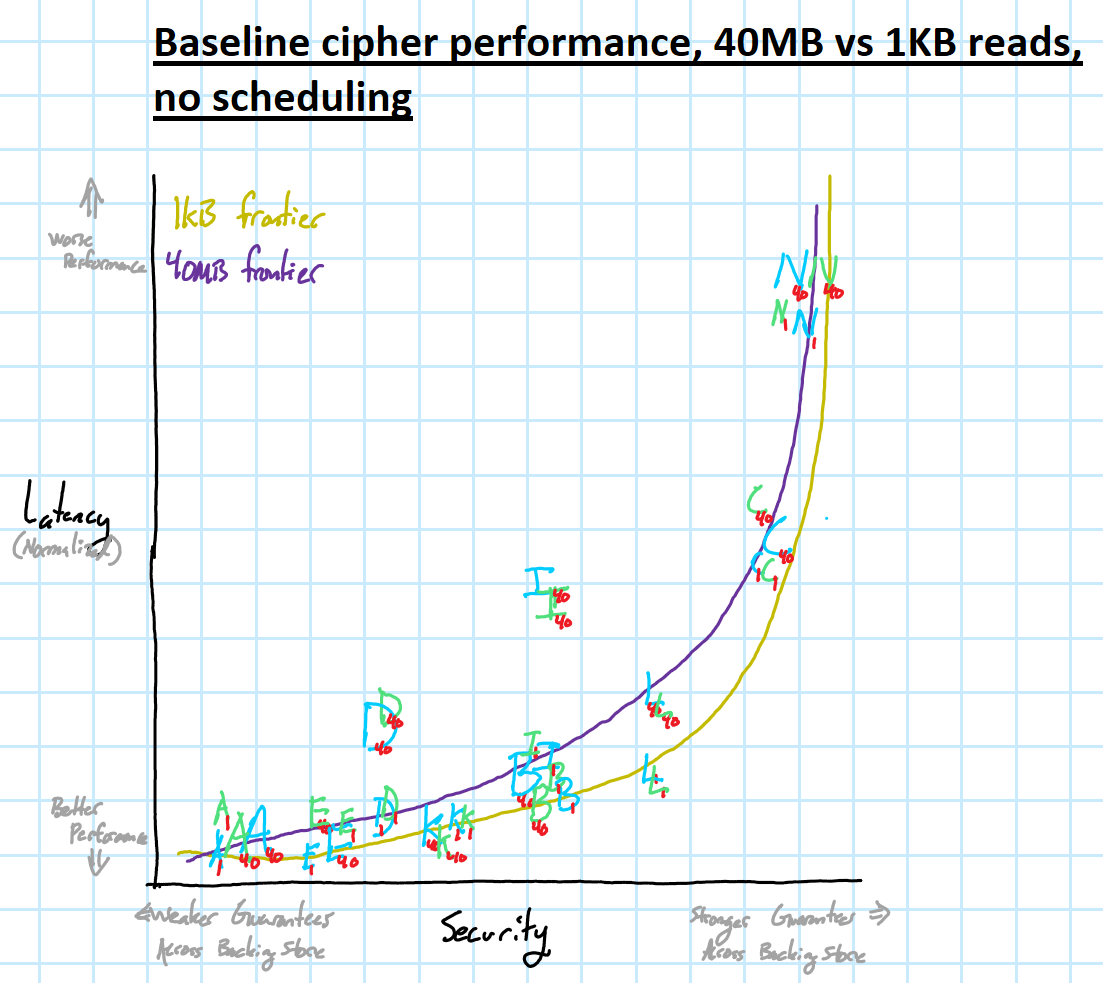
\includegraphics[width=\linewidth]{drawn/2.png}
   \caption{\TODO{Caption goes here}\TODO{Necessary chart? Or should we punt it to the dissertation and simply explain somewhere that the curves are congruent with the original?}}\label{fig:40mb-vs-1kb-read}
\end{figure}

\begin{figure}[ht]
 \centering
  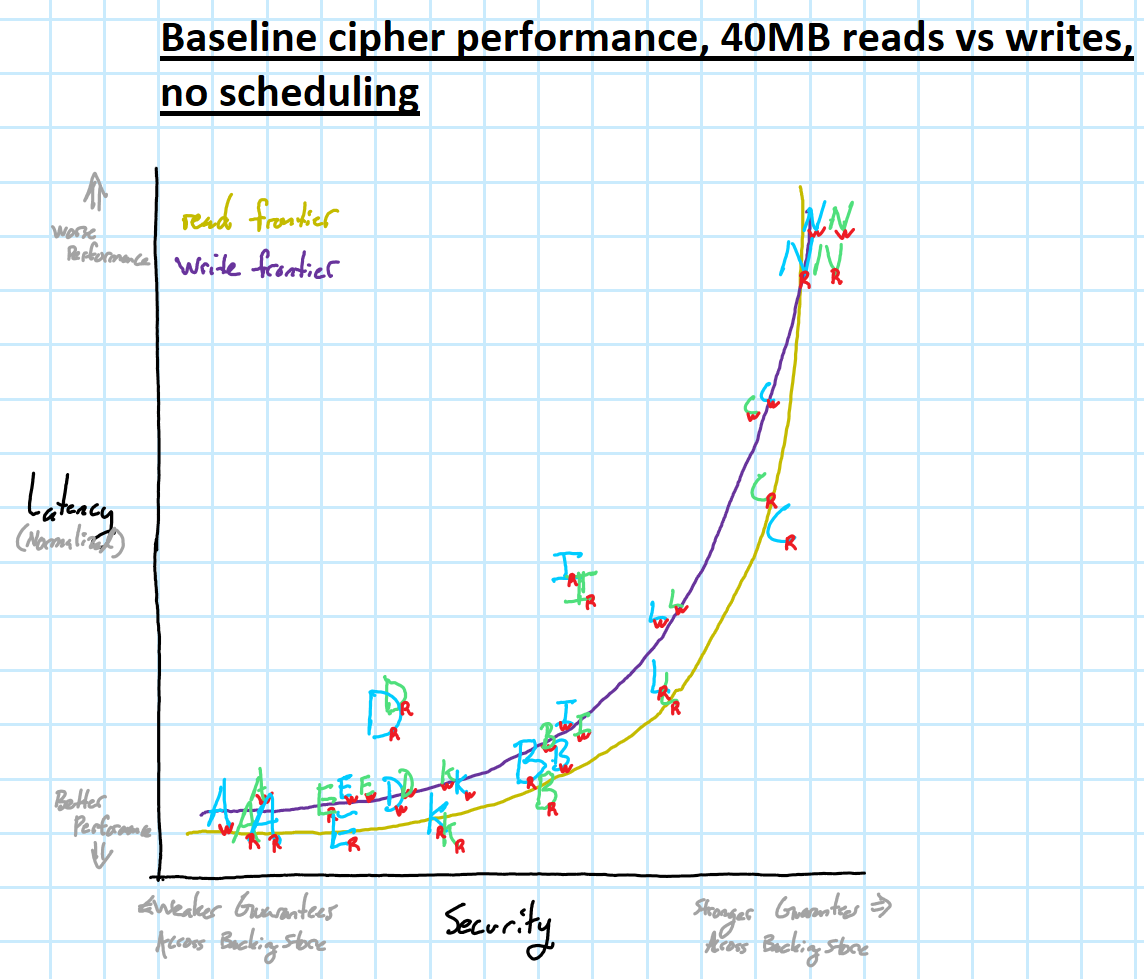
\includegraphics[width=\linewidth]{drawn/3.png}
   \caption{\TODO{Caption goes here}\TODO{Necessary chart? Or should we punt it to the dissertation and we simply explain somewhere that the curves are congruent with the original?}}\label{fig:40mb-read-vs-write}
\end{figure}}

\begin{figure}[ht]
 \centering
  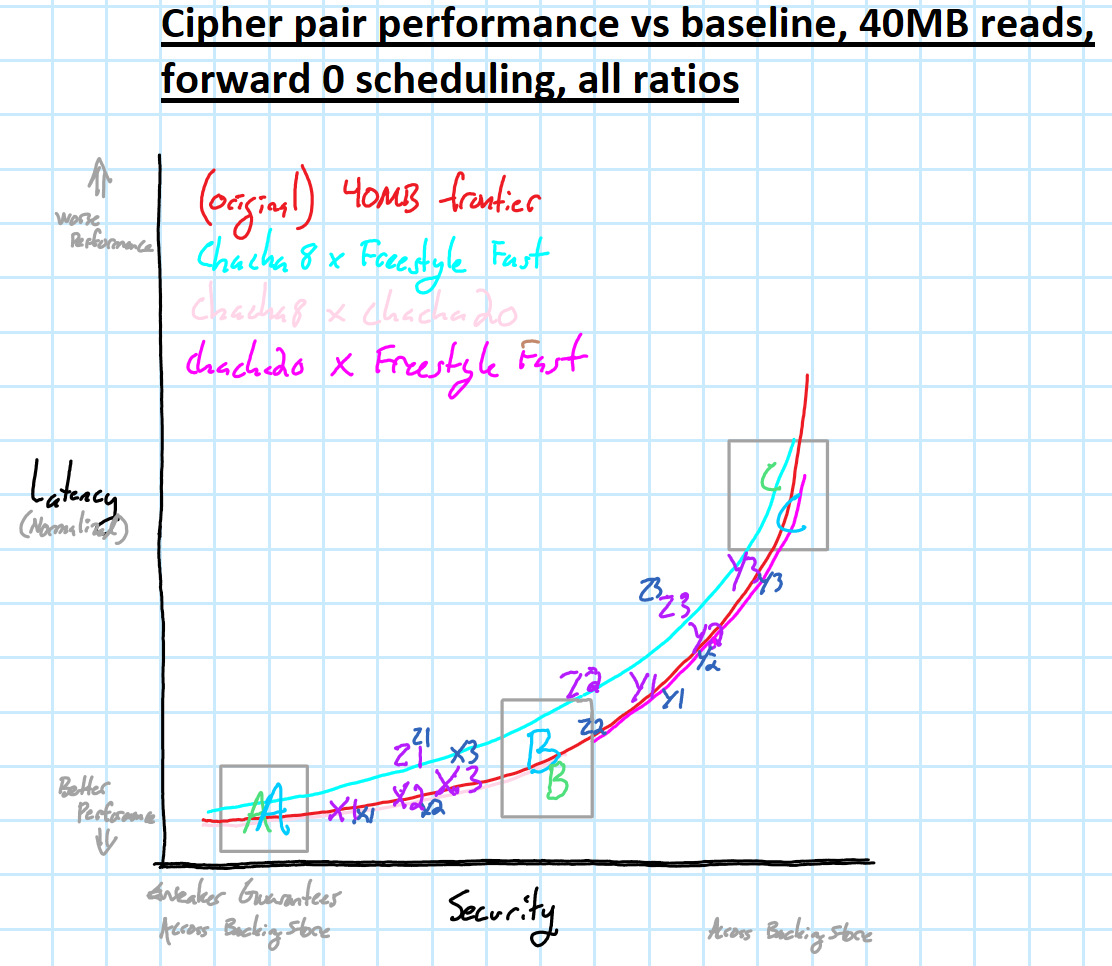
\includegraphics[width=\linewidth]{drawn/4.png}
   \caption{\TODO{Caption goes here}}\label{fig:navigating-the-space}
\end{figure}

\figref{navigating-the-space} shows the 40MB read performance of three ciphers:
ChaCha8, ChaCha20, and Freestyle in its "fast" configuration. This illustrates
the tradeoff space between latency/energy and security for these three static
discrete pareto optimal configurations achievable offline via prior work.
\figref{navigating-the-space} additionally illustrates the flexibility of
SwitchBox using the 0-forward switching strategy to reach pareto optimal dynamic
configuration points \emph{between} traditional static configuration in the
tradeoff space that are unachievable via prior work.

\TODO{Should there be a "ciphers" section somewhere that describes all the
various ciphers and cipher configurations? Would that best go in the design
section? Or perhaps here in the evaluation?} \TODO{It should probably be in methodology or setup.  You can save some space by mentioning them all in the motivation section and then referring back to that list here.  It is also a little surprising that only three end up being pareto-optimal, so that is worth a sentence or two of discussion.}

\begin{figure}[ht]
 \centering
  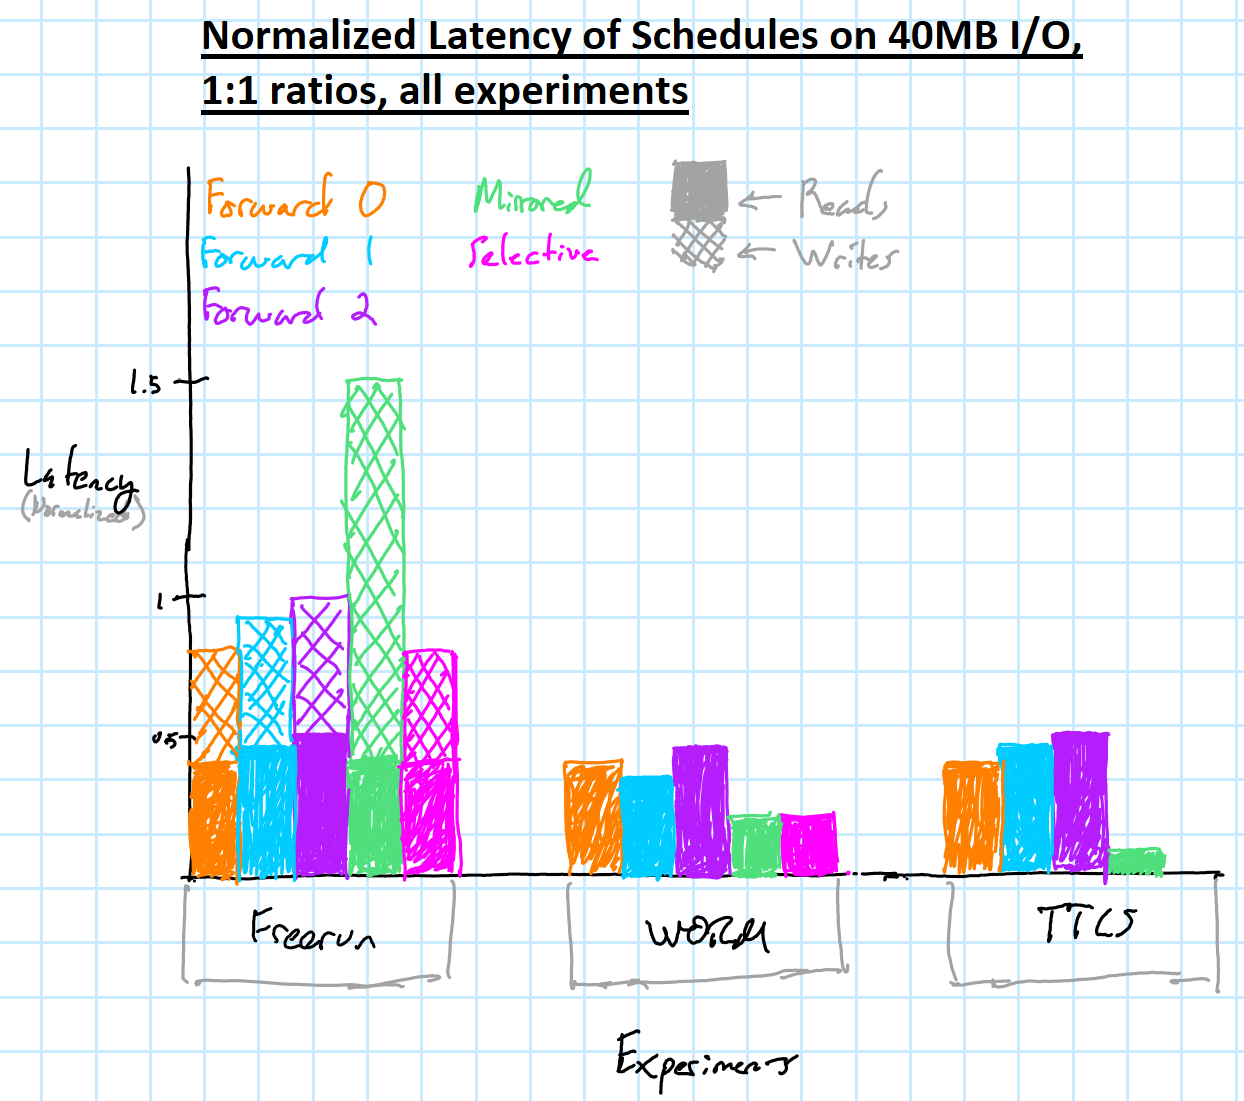
\includegraphics[width=\linewidth]{drawn/9.png}
   \caption{\TODO{Caption goes here}}\label{fig:strategy-vs-strategy}
\end{figure}

\figref{strategy-vs-strategy} show the the performance of forward, mirrored, and
selective strategies against two 40MB read and write workloads: Freerun and
WORM. \TODO{Explain these two workloads.} Additionally, the time required to
transition the entire backing store from one cipher to the other is included
\TODO{This is "time to cipher switch" or TTCS, but this is renamed in the actual
figure.}

1-forward and 2-forward have overhead that makes them slower than forward 0 for
sequential and random freerun. However, WORM workload shows 1-forward
outperforming 0-forward by \TODO{include percentage (it's small)}. This is
because WORM workload characteristics allow benefits of more aggressive forward
switching to be realized \TODO{Elaborate more here}.

The mirrored and selective switching strategies achieve read parity with the
static cipher configurations, hence their performance. However, mirrored stacks
write latency of both ciphers in the pair because writes are mirrored across
both partitions. On the other hand, selective switching achieves write parity
with the static configuration. Mirrored and selective are not preferable to
forward in all circumstances because drive space is traded off; in our
experiments, half the drive is lost to partitioning.

\TODO{Word these paragraphs better. Include numbers from chart to be more
specific.}

Selective is usually preferable to mirrored due to mirrored strategy's egregious
write overhead. However, forward and selective take a comparatively long time to
transition the entire backing store from one cipher to the other while mirrored
can achieve this virtually instantaneously. If it is not desirable to maintain
both encrypted versions of data on the backing store, one partition or the other
can be TRIM-ed and the data deleted relatively quickly. On the other hand, when
using the selective strategy, it is not possible to transition the backing store
entirely to one cipher or another (hence no bar for TTCS). For the forward
strategy, it takes a long time. \TODO{Specific numbers from chart need to go in
here.}

\TODO{Perhaps explain a bit more about when one cipher is preferable to another?
Or do the previous paragraphs hit on this enough already? Hopefully we're not
bumping up against the page limit yet...}
